\documentclass[11pt]{beamer}
\usepackage[utf8]{inputenc}
\usepackage[T1]{fontenc}
\usepackage{lmodern}
\usetheme{default}
	\usefonttheme[onlymath]{serif}

\usepackage{graphicx}
	\graphicspath{{Pictures/}}
\usepackage{subfig}
\captionsetup[subfloat]{labelformat=empty}
\captionsetup[figure]{labelformat=empty}

\usepackage{booktabs} % per le tabelle, permette di usare \toprule ecc
\usepackage{amsmath}
\usepackage{mathtools}
\usepackage{multimedia}
\usepackage{hyperref}
\usepackage{ifxetex}
\ifxetex
	\usepackage{fontspec}
	\setsansfont[Scale=0.95]{Arial}
\fi

\setbeamertemplate{footline}[frame number]

\begin{document}
	\author{Alessio Raimondi}
	\title{Calibration of snowflake shape parameters}
	\begin{frame}[plain]
		\maketitle
	\end{frame}
		
	\begin{frame}{Data Analysis Background}
		\begin{block}{Bayes' Theorem}
			\begin{equation*}
				\underbrace{prob(HP|D,I)}_{Posterior Probability} \propto
				\underbrace{prob(D|HP,I)}_{Likelihood Function} \cdot \underbrace{prob(HP|I)}_{Prior Probability}
			\end{equation*}
			\begin{itemize}
				\item \textbf{Prior:} State of knowledge (or ignorance) before analyzing the data 
				
				\item \textbf{Likelihood:} Experimental measurements
				\item \textbf{Posterior:} State of knowledge in light of the data
			\end{itemize}
		\end{block}
		\begin{block}{Marginalization Equation + Sum Rule}
			\begin{equation*}
				prob(HP|D,I) = \int_{-\infty}^{+\infty} prob(HP,X|D,I) dX = 1
			\end{equation*}
			where $ X $ must be a (continuous) set of \textit{mutually exclusive} and \textit{exhaustive} possibilities (independent variable of model calibration)
		\end{block}
	\end{frame}

	\begin{frame}{Single Parameter Estimation}
		\centering
		\includegraphics[width=\textwidth, keepaspectratio] {SingleParameter.pdf}
		\begin{itemize}
			\item $ (d_v, v_t) $: Experimental data
			\item $ \varphi $: Free parameter
		\end{itemize}
	\end{frame}

	\begin{frame}{Problem formulation 1/2}
		\begin{block}{Prior}
			\begin{equation*}
				prob(HP|I) = prob(\varphi) = \left\{ 
				\begin{array}{cc}
					\dfrac{1}{\varphi_{max} - \varphi_{min}} & \text{for} \quad \varphi_{min} < \varphi < \varphi_{max}\\
					0 & otherwise
				\end{array} \right.
			\end{equation*}	
		\end{block}
	
		\begin{block}{Likelihood}
			\begin{equation*}
				prob(D|HP,I) = prob(\{d_v, v_t\}|\varphi) = 
				\prod_{k = 1}^{N_{data}} e^{-\dfrac{1}{2} \left(\dfrac{v_{t,k} - v_t(d_{v,k}, \varphi)}{\sigma_k} \right)^2}
			\end{equation*}
		\end{block}
	\end{frame}

	\begin{frame}{Problem formulation 2/2}
		\begin{block}{Governing Equation}
			\begin{equation*}
				\frac{1}{2} \rho_a v_t^2 S_{\perp} c_D(Re, \varphi, \text{model}) = (\rho_s(\frac{d_v}{den}) - \rho_a) V g
			\end{equation*}
			by defining the Aspect Ratio $ := A_r = V / S_{\perp} $
			\begin{equation*}
				\frac{1}{2} v_t^2 c_D(Re, \varphi, \text{model}) = \dfrac{\rho_a - \rho_s(d_v)}{\rho_a} g A_r
			\end{equation*}
			and must be solved iteratively.
		\end{block}
	\end{frame}

	\begin{frame}{Model: Chien - 1994}
		Simple model (only 1 free parameter), just for method testing.\\
		Free parameter: Sphericity $ \varphi = \Phi $
		\begin{equation*}
			c_D = \frac{30}{Re} + 67.289 e^{-5.05 \Phi}
		\end{equation*}
		\begin{equation*}
			A_r = \dfrac{V}{S_{\perp}} = \dfrac{\dfrac{\pi}{6} d_v^3}{\dfrac{\pi d_v}{\Phi}} = \dfrac{1}{6} d_v \Phi
		\end{equation*}
		\textbf{Obs}. Here $ S_{\perp} $ has been replaced with just $ S $ (particle surface area) because the available shape parameter ($ d_v, \Phi $) could not describe all the needed geometrical characteristics of the particle.
	\end{frame}

	\begin{frame}{Results 1/2}
		\centering
		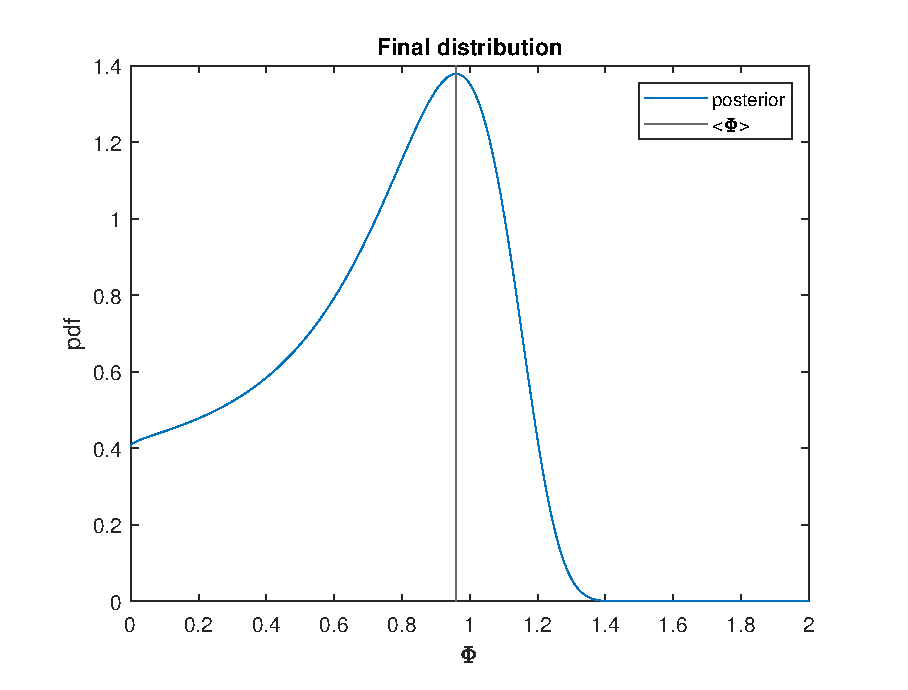
\includegraphics[width=\linewidth]{ChienPost.eps}
	\end{frame}

	\begin{frame}{Results 2/2}
		\centering
		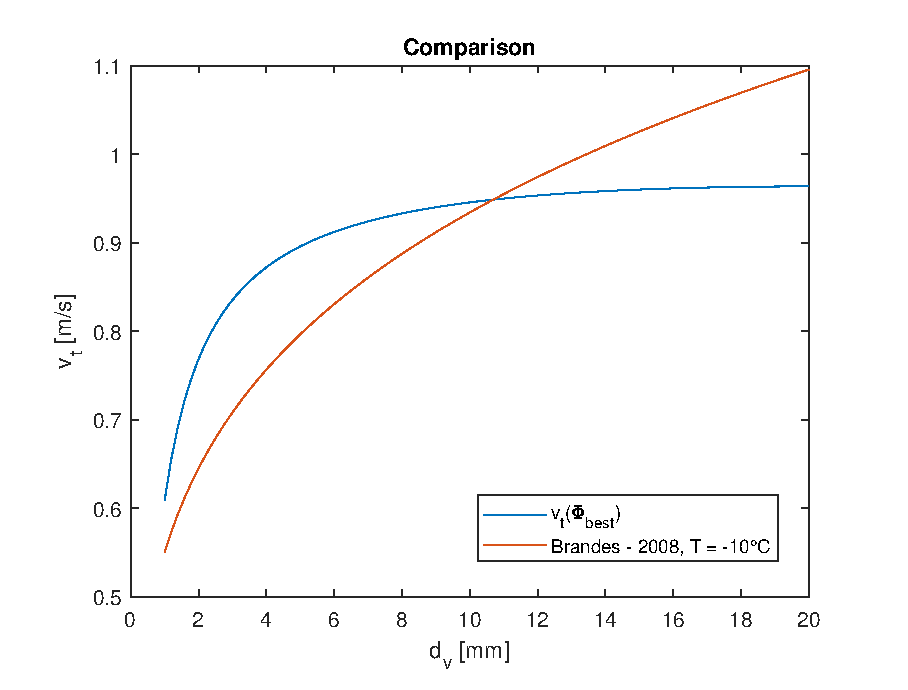
\includegraphics[width=\linewidth]{ChienComparison.eps}
	\end{frame}

% -------------------------------------------------------------------------------
	\begin{frame}{Double Parameter Estimation}
		\centering
		\includegraphics[width=\textwidth, keepaspectratio] {DoubleParameter.pdf}
		\begin{itemize}
			\item $ (d_v, v_t) $: Experimental data
			\item $ \varphi_1, \varphi_2 $: Free parameters
		\end{itemize}
	\end{frame}
	
	\begin{frame}{Problem formulation 1/2}
		\begin{block}{Prior}
			\begin{equation*}
				prob(HP|I) = prob(\varphi_1, \varphi_2) = \left\{ 
				\begin{array}{cc}
				\dfrac{1}{(\varphi_{1, max} - \varphi_{1, min}) (\varphi_{2, max} - \varphi_{2, min})} & \text{for} \quad \varphi_{1, min} < \varphi_1 < \varphi_{1, max} and \varphi_{2, min} < \varphi_2 < \varphi_{2, max}\\
				0 & otherwise
				\end{array} \right.
			\end{equation*}	
		\end{block}
		
		\begin{block}{Likelihood}
			\begin{equation*}
				prob(\{d_v, v_t\}|\varphi_1, \varphi_2) = 
				\prod_{k = 1}^{N_{data}} e^{-\dfrac{1}{2} \left(\dfrac{v_{t,k} - v_t(d_{v,k}, \varphi_1, \varphi_2)}{\sigma_k} \right)^2}
			\end{equation*}
		\end{block}
	\end{frame}
	
	\begin{frame}{Problem formulation 2/2}
		\begin{block}{Governing Equation}
			\begin{equation*}
				\frac{1}{2} \rho_a v_t^2 S_{\perp} c_D(Re, \varphi_1, \varphi_2, \text{model}) = (\rho_s(d_v) - \rho_a) V g
			\end{equation*}
			by defining the Aspect Ratio $ := A_r = V / S_{\perp} $
			\begin{equation*}
				\frac{1}{2} v_t^2 c_D(Re, \varphi_1, \varphi_2, \text{model}) = \dfrac{\rho_a - \rho_s(d_v)}{\rho_a} g A_r
			\end{equation*}
			and must be solved iteratively.
		\end{block}
	\end{frame}

	\begin{frame}{Model: Ganser - 1993  1/2}
		Free parameters:
		\begin{itemize}
			\item Sphericity $ \varphi_1 = \Phi $
			\item Diameter Ratio $ \varphi_2 = d_n / d_v $
		\end{itemize}
		\vfill
		\begin{equation*}
			c_D = K_2 \left( \frac{24}{Re K_1 K_2} (1 + 0.1118 (Re K_1 K_2)^{0.6567}) + \frac{0.4305}{1 + \frac{3305}{Re K_1 K_2}}\right) 
		\end{equation*}
		
		\begin{equation*}
			A_r = \dfrac{V}{S_{\perp}} = \dfrac{\dfrac{\pi}{6} d_v^3}{\dfrac{\pi}{4} d_n^2} = \dfrac{2}{3} \dfrac{d_v^3}{d_n^2}
		\end{equation*}
	\end{frame}
	
	\begin{frame}{Model: Ganser - 1993  2/2}
		\begin{block}{Stokes' shape factor}
			\begin{equation*}
			K_1 = \left( \frac{1}{3} \frac{d_n}{d_v} + \frac{2}{3} \Phi^{-\frac{1}{2}} \right)^{-1} 
			\end{equation*}
		\end{block}
		\begin{block}{Newton's shape factor}
			\begin{equation*}
			K_2 = 10^{1.8148 (-log(\Phi))^{0.5743}}
			\end{equation*}
		\end{block}
	\end{frame}
	
	\begin{frame}{Results 1/2}
		\centering
		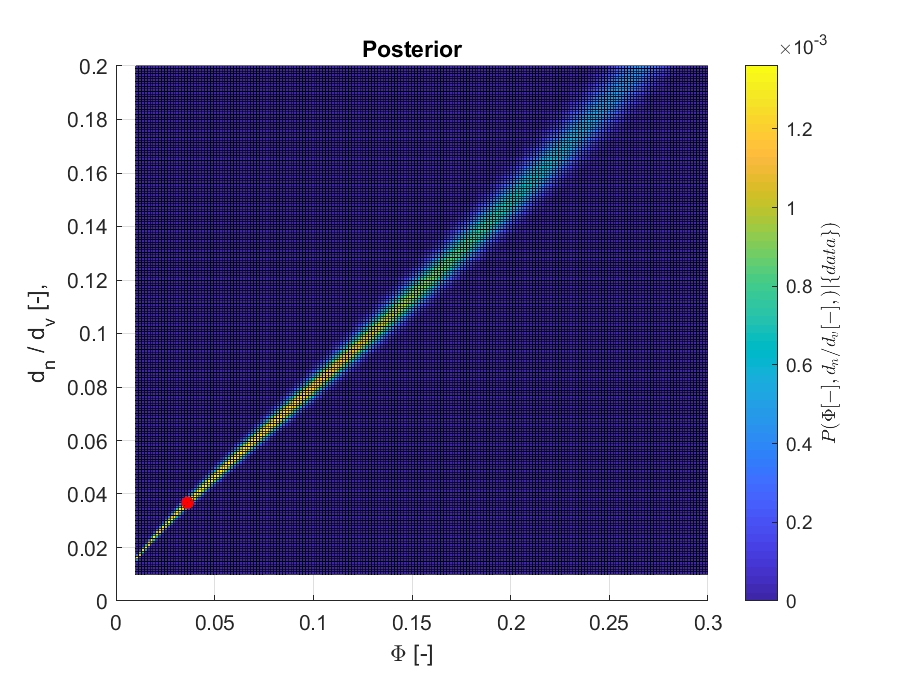
\includegraphics[width=\linewidth]{GanserPost.eps}
	\end{frame}
	
	\begin{frame}{Results 2/2}
		\centering
		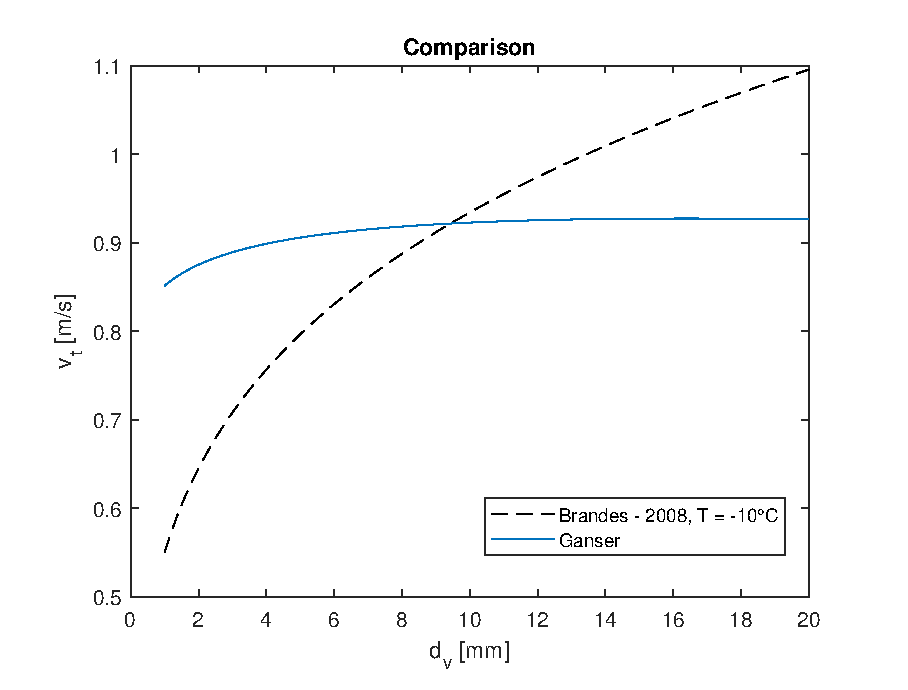
\includegraphics[width=\linewidth]{GanserComparison.eps}
	\end{frame}

	\begin{frame}{Ganser Study 1/2}
		\centering
		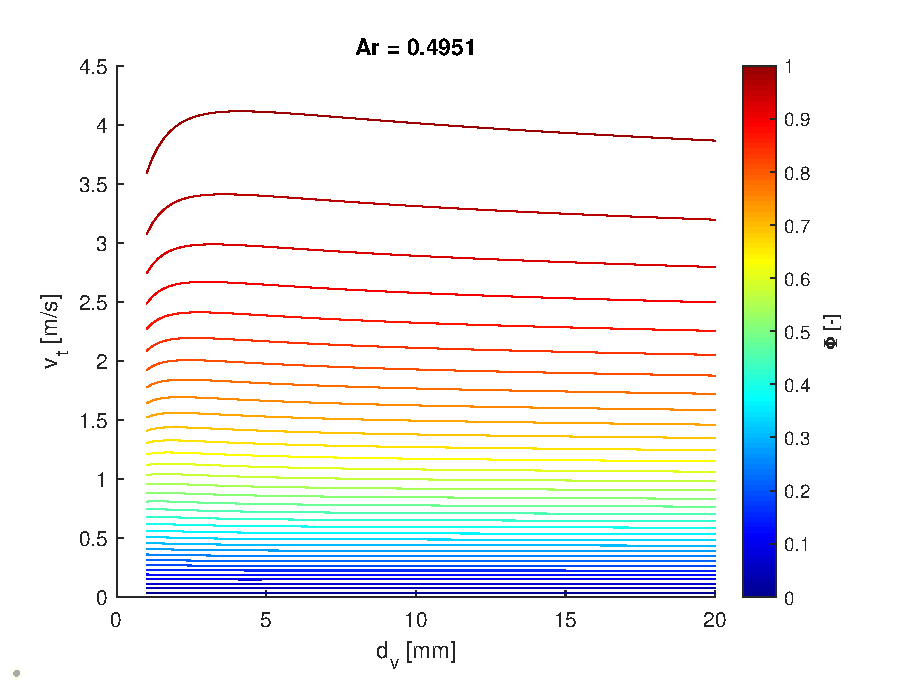
\includegraphics[width=\linewidth]{GanserStudy.eps}
	\end{frame}

	\begin{frame}{Ganser Study 2/2}
		\centering
		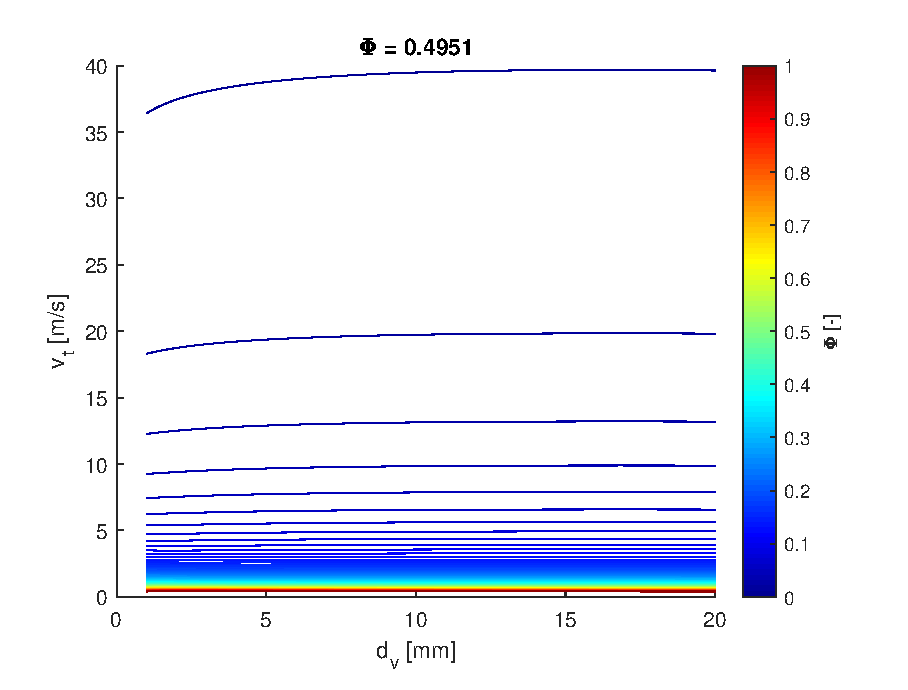
\includegraphics[width=\linewidth]{GanserStudy2.eps}
	\end{frame}

		\begin{frame}{Holtzer and Sommerfeld Study 1/2}
		\centering
		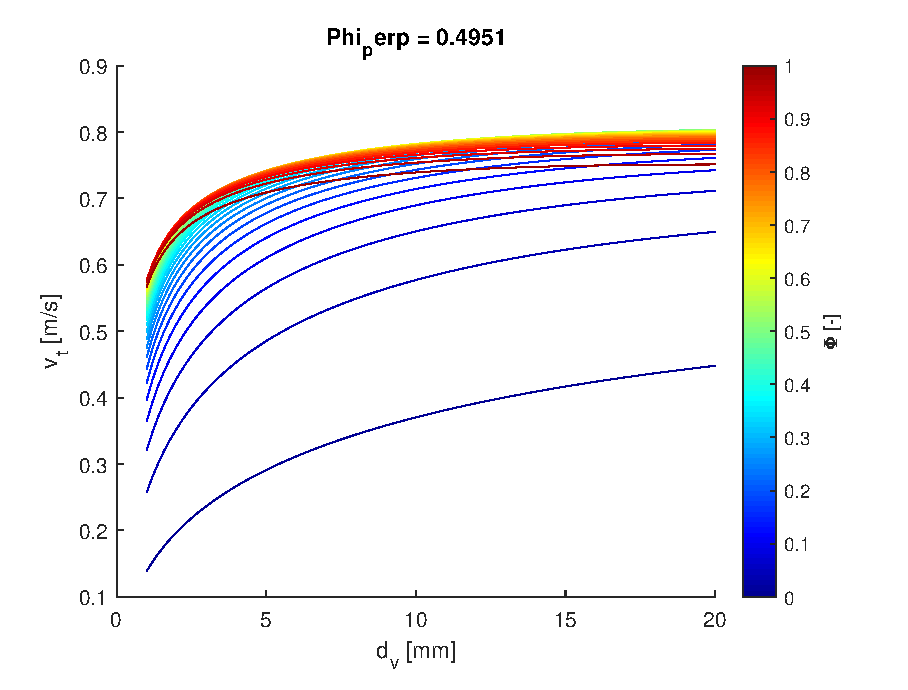
\includegraphics[width=\linewidth]{HoltzerSommerfeldStudy.eps}
	\end{frame}
	
	\begin{frame}{Holtzer and Sommerfeld Study 2/2}
		\centering
		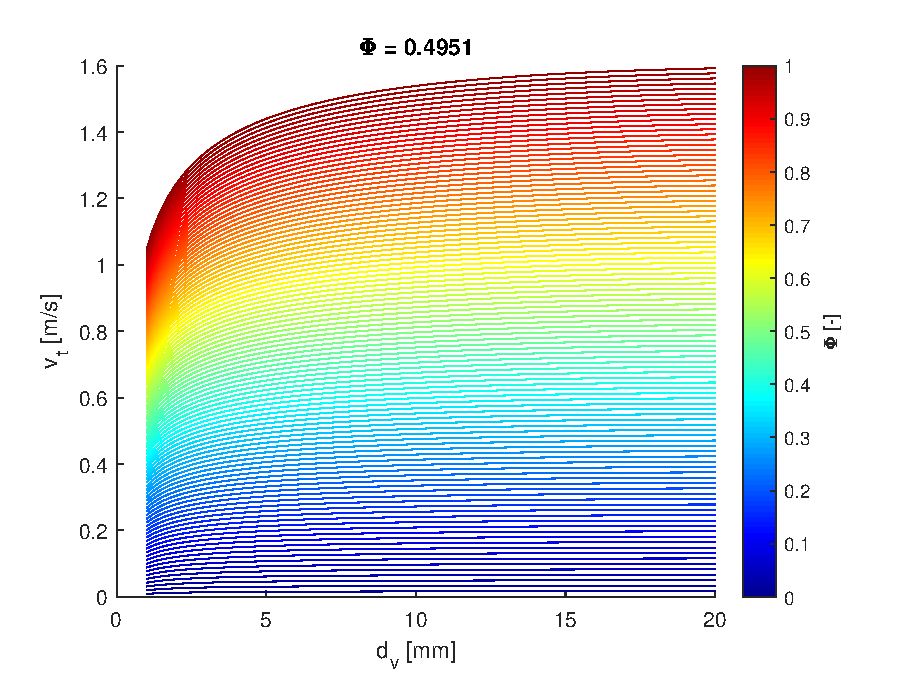
\includegraphics[width=\linewidth]{HoltzerSommerfeldStudy2.eps}
	\end{frame}
	
\end{document}
